\section{Evaluation}
\label{sec:eval}

В данном разделе мы рассмотрим семантику с предикатом, основанном на структурной рекурсии. Также мы представим результаты апробации семантики с тремя разными предикатам на наборе примеров. Для апробации семантика была реализована на языке \textsc{Haskell} в виде интерпретатора. 


% Имперически подобранный критерий
В качестве предиката нам необходим критерий, отличающий вызов, который выгодно раскрутить сейчас от вызова, который стоит отложить. Мы предлагаем predicate by well-quasi-ordering, который эффективен для структурно-рекурсивных отношений. У таких отношений есть хотя бы один аргумент, который структурно убывает с каждым шагом рекурсии. Перестаёт убывать такой аргумент, только когда свободные переменные, которые он содержит, начинают уточняться. И когда все структурные агументы перестанут убывать, мы будем останавливать развёртку вызова.

Сначала определим отношение на кортежах термов.

\begin{definition}
Пусть $t_1^1, \ldots, t_n^1, \, t_1^2, \ldots, t_n^2 \in \mathcal{T}_{\mathcal A}$. Если для любого $i$ верно, что $height(t_i^1) \leq height(t_i^2)$, и существует $j$, для которого $height(t_i^1) < height(t_i^2)$, тогда 
\[
  (t_1^1, \ldots, t_n^1) \leq_h (t_1^2, \ldots t_n^2).
\]
\end{definition}

Отношение ``$\leq_h$'' сравнивает термы по их высоте. Оно требует, чтобы хотя бы один терм левого кордежа был строго короче, чем соответствующий терм из правого кортежа. Остальные левые термы должны быть не длиннее соотвествующих термов в правом кортеже.

\begin{lemma}
\label{lemma:wqo1}
Отношение ``$\leq_h$'' является well-quasi-ordering.
\end{lemma}
Доказывается индукцией по сумме высот всех термов.

Теперь определим отношение на парах из подстановки и реляционного применения.

\begin{definition}
Пусть $\theta_1, \theta_2$ --- подстановки,  $r_1, r_2$ --- реляционные применения. Если $r_1 = R(t^1_1,\,\ldots,\,t^1_n)$, $r_2 = R(t^2_1,\,\ldots,\,t^2_n)$, $j_1, \ldots, j_k$ --- номера структурно-рекурсивных аргументов реляционного отношения $R$ и $(\theta_1 t^1_{j_1}, \ldots, \theta_1 t^1_{j_k}) \leq_h (\theta_2 t^2_{j_1}, \ldots, \theta_2 t^2_{j_k})$, тогда
\[
  (\theta_1, r_1) \leq_{sr} (\theta_2, r_2).
\]
\end{definition}

Отношение ``$\leq_{sr}$'' сравнивает только структурно-рекурсивные аргументы двух вызовов одного отношения по высоте с помощью определенного вышe ``$\leq_h$''.

\begin{lemma}
Отношение ``$\leq_{sr}$'' является well-quasi-ordering.
\end{lemma}
Следует из леммы~\ref{lemma:wqo1}.

А значит семантика с $pred_{\leq_{sr}}$ является справедливой по теореме~\ref{todo}.

\begin{figure*}
\centering
\begin{minipage}{.5\textwidth}
  \centering
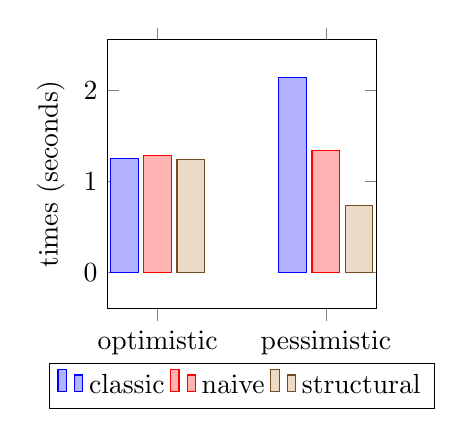
\begin{tikzpicture}
\begin{axis}[
    ybar, ymax = 2, ymin = 0.15,
    enlargelimits=0.3,
    width=5cm, height=5cm,
    legend style={at={(0.5,-0.2)},
      anchor=north,legend columns=-1},
    ylabel={times (seconds)},
    symbolic x coords={optimistic, pessimistic},
    xtick=data
    ]
\addplot coordinates {(optimistic,1.254) (pessimistic,2.142)};
\addplot coordinates {(optimistic,1.282) (pessimistic,1.337)};
\addplot coordinates {(optimistic,1.236) (pessimistic,0.733)};
\legend{classic,naive,structural}
\end{axis}
\end{tikzpicture}
 \captionof{figure}{revers$^o$ forward evaluation \\ for a list with a length of 90}
  \label{fair:plot-reverso}
\end{minipage}%
\begin{minipage}{.5\textwidth}
  \centering
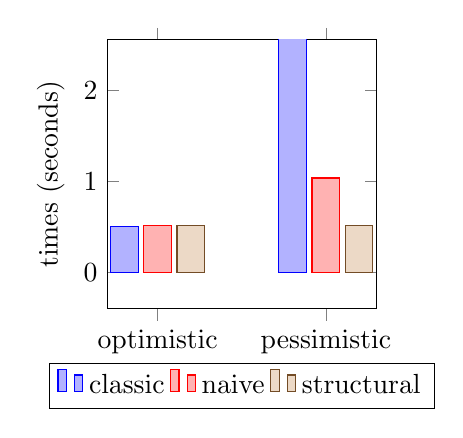
\begin{tikzpicture}
\begin{axis}[
    ybar, ymax = 2, ymin = 0.15,
    enlargelimits=0.3,
    width=5cm, height=5cm,
    legend style={at={(0.5,-0.2)},
      anchor=north,legend columns=-1},
    ylabel={times (seconds)},
    symbolic x coords={optimistic, pessimistic},
    xtick=data
    ]
\addplot coordinates {(optimistic,0.504) (pessimistic,300)};
\addplot coordinates {(optimistic,0.508) (pessimistic,1.035)};
\addplot coordinates {(optimistic,0.513) (pessimistic,0.513)};
\legend{classic,naive,structural}
\end{axis}
\end{tikzpicture}
 \captionof{figure}{sort$^o$ forward evaluation \\ for a list with a length of 5}
\label{fair:plot-sorto}
\end{minipage}
\end{figure*}

\begin{figure*}
\centering
\begin{minipage}{.5\textwidth}
  \centering
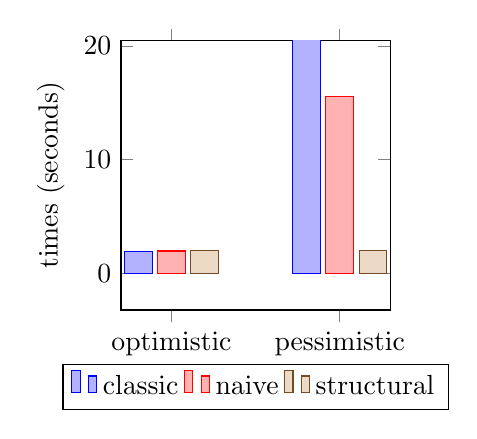
\begin{tikzpicture}
\begin{axis}[
    ybar, ymax = 16, ymin = 1.2,
    enlargelimits=0.3,
    width=5cm, height=5cm,
    legend style={at={(0.5,-0.2)},
      anchor=north,legend columns=-1},
    ylabel={times (seconds)},
    symbolic x coords={optimistic, pessimistic},
    xtick=data
    ]
\addplot coordinates {(optimistic,1.909) (pessimistic,300)};
\addplot coordinates {(optimistic,1.945) (pessimistic,15.516)};
\addplot coordinates {(optimistic,1.980) (pessimistic,1.978)};
\legend{classic,naive,structural}
\end{axis}
\end{tikzpicture}
 \captionof{figure}{``The Tower of Hanoi'' \\ solver evaluation}
\label{fair:plot-hanoi}
\end{minipage}%
\begin{minipage}{.5\textwidth}
  \centering
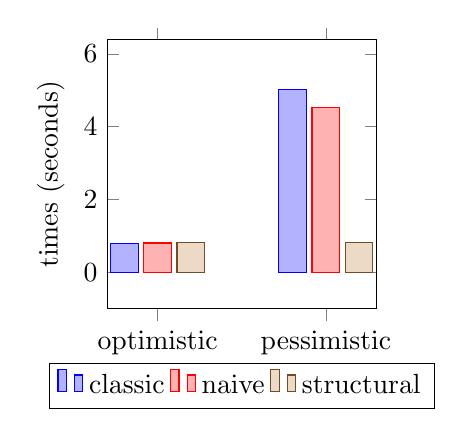
\begin{tikzpicture}
\begin{axis}[
    ybar, ymax = 5, ymin = 0.375,
    enlargelimits=0.3,
    width=5cm, height=5cm,
    legend style={at={(0.5,-0.2)},
      anchor=north,legend columns=-1},
    ylabel={times (seconds)},
    symbolic x coords={optimistic, pessimistic},
    xtick=data
    ]
\addplot coordinates {(optimistic,0.783) (pessimistic,5.019)};
\addplot coordinates {(optimistic,0.801) (pessimistic,4.522)};
\addplot coordinates {(optimistic,0.812) (pessimistic,0.817)};
\legend{classic,naive,structural}
\end{axis}
\end{tikzpicture}
 \captionof{figure}{``Bridge and torch problem'' \\ solver evaluation}
\label{fair:plot-bridge}
\end{minipage}
\end{figure*}

Now we will discuss evaluation. Целью эвалюации является выявления влияния порядка конъюнктов на эффективность трех различных семантик.

Первая семантика с предикатом $pred_{\mbox{\lstinline{true}}}$ близка к классическим реализациям \mk. В дальнейшем будем называть её {\bf left-biased}.

Вторая семантика с предикатом $pred_N$ соответсвует равномерному вычислению всех конъюнктов. Эту семантику будем назвать {\bf naive}.

Третья семантика с предикатом $pred_{\leq_{sr}}$ вычисляет структурно-рекурсивные конъюнкты, пока убывают структурно-рекурсивные аргументы. Её будем называть {\bf structural}.

For evaluation we've chosen two simple programs (list reversing and list sorting) and three more complicated (the ``Hanoi Towers''\footnote{\url{https://en.wikipedia.org/wiki/Tower_of_Hanoi}} solver, the
``Bridge and torch problem''\footnote{\url{https://en.wikipedia.org/wiki/Bridge_and_torch_problem}} solver and ``Water pouring puzzle''\footnote{\url{https://en.wikipedia.org/wiki/Water_pouring_puzzle}} solver).
% Для каждой программы мы сделали две версии. Оптимистичная версия --- это программа, в которой мы вручную подобрали оптимальный порядок конъюнктов и пессиместичная версия --- программа с неоптимальным порядком конъюнктов. В последующих диаграммах и таблице указаны средние значения 10 запусков тестов. Также для наивной равномерной конъюнкции мы подобрали количество разверток вручную. Для равномерной конъюнкции, основанной на структурной рекурсии, N было фиксировано и равно 100.
Each program was written in two versions: ``optimistic'' (with the order of important conjuncts set to provide the best performance) and ``pessimistic'' (with the order of important
conjuncts set to provide the worst performance). Also we evaluated list reversing and list sorting in both directions. In the case of the list reversing, queries \lstinline{(revers$^o$ [1;2;3] q)} and \lstinline{(revers$^o$ q [1;2;3])}\! will give the same answer \lstinline{q = [3;2;1]} but the ``optimistic'' order of conjuncts is different for them. In the case of list sorting, queries \lstinline{(sort$^o$ [1;2;3] q)} and \lstinline{(sort$^o$ q [1;2;3])} will give different answers. The first one gives sorted list \lstinline{q = [1;2;3]}, the second one gives all permutations of list \lstinline{[1;2;3]}\!\!. 

All benchmarks were run ten times, and the average time was taken. For the naive  semantics we cherry-picked the best value of unfolding bound manually. Structural arguments for each relations were detected automatically.

% На изображениях 12-15 представлены результаты апробации в виде столбцовых диаграмм. В оптимистичном случае результаты схожи для всех семантик. В пессиместичном случае время работы напрпавленной конъюнкции резко возрастает, время работы наивной равномерной конъюнкции также ворзрастает, но не так сильно. Равномерная конъюнкция, основанная на структурной рекурсии, демострирует схожую эффективность в сравнении с оптимистичным случаем.
Fig.~\ref{fair:plot-reverso}-\ref{fair:plot-bridge} show the results of evaluation in the form of bar charts. In the optimistic case, the results are similar for all semantics.
In the pessimistic case the evaluation time of the directed conjunction rapidly increases, the evaluation time of the naive fair conjunction also increases, but not so much.
The fair semantics based on structural recursion demonstrates a similar efficiency as in the optimistic case.

\begin{figure*} %[h!]
  \small
  \centering
  \begin{tabular}{ c | c | c | c | c | c | c | c }
    \multirow{2}{*}{relation} & \multirow{2}{*}{size} & 
    \multicolumn{2}{c}{left-biased semantics} &
    \multicolumn{2}{c}{naive semantics} &
    \multicolumn{2}{c}{structural semantics} \\
    \cline{3-8}
    & & optimistic & pessimistic & optimistic & pessimistic & optimistic & pessimistic  \\ 
    \hline
    \multirow{3}{*}{\begin{tabular}{c} forward \\ revers$^o$ \end{tabular}}
                 & 30   & 0.527 & 0.587  & 0.532 & 0.595   & 0.539 & 0.532 \\
                 & 60   & 0.639 & 0.947  & 0.643 & 0.790   & 0.657 & 0.577 \\
                 & 90   & 1.254 & 2.142  & 1.282 & 1.337   & 1.236 & 0.733 \\
    \hline
    \multirow{3}{*}{\begin{tabular}{c} backward \\ revers$^o$ \end{tabular}}
                 & 30   & 0.531 & 0.579  & 0.547 & 0.570  & 0.553 & 0.563 \\
                 & 60   & 0.655 & 0.875  & 0.667 & 0.812  & 0.668 & 0.681 \\
                 & 90   & 1.316 & 1.813  & 1.327 & 1.503  & 1.360 & 1.359 \\
    \hline
    \multirow{5}{*}{\begin{tabular}{c} forward \\ sort$^o$ \end{tabular}}
                 & 3    & 0.467 & 0.503  & 0.474 & 0.481  & 0.472 & 0.479 \\
                 & 4    & 0.484 & 4.679  & 0.485 & 0.493  & 0.490 & 0.488 \\
                 & 5    & 0.504 & $>$300 & 0.508 & 1.035  & 0.513 & 0.513 \\
                 & 6    & 0.526 & $>$300 & 0.237 & 14.369 & 0.544 & 0.547 \\
                 & 30   & 1.915 & $>$300 & 1.936 & $>$300 & 1.983 & 1.987 \\
    \hline
    \multirow{4}{*}{\begin{tabular}{c} backward \\ sort$^o$ \end{tabular}}
                 & 3    & 0.518 &  0.519 & 0.518 & 0.521  & 0.520 & 0.521 \\
                 & 4    & 0.533 &  0.856 & 0.534 & 0.540  & 0.534 & 0.537 \\
                 & 5    & 0.680 & 93.914 & 0.713 & 1.528  & 0.718 & 0.714 \\
                 & 6    & 2.931 & $>$300 & 2.947 & 59.647 & 2.938 & 2.936 \\
    \hline
    hanoi$^o$    & -    & 1.909 & $>$300 & 1.945 & 15.516 & 1.980 & 1.978 \\
    \hline
    bridge$^o$   & -    & 0.783 & 5.019  & 0.801 & 4.522  & 0.812 & 0.817 \\
    \hline
    water$^o$    & -    & 3.513 & $>$300 & 3.518 & $>$300 & 3.538 & 3.771

  \end{tabular}
  \caption{The results of evaluation: running times of benchmarks in seconds}
  \label{fair:evaluation-table}
\end{figure*}

% Более подробно результаты представлены на изображении 16. Можно заметить, что время работы программы sorto в пессиместичном случае очень быстро растет с увеличением длины списка для направленной конъюнкции и наивной равномерной. В случае с равномерной конъюнкцией, основанной на структурной рекурсии, пессиместичный случай растет сопостовимо с оптимистичным.
The results are presented in more detail in Fig.~\ref{fair:evaluation-table}. ``Hanoi Towers'' solver has name \lstinline{hanoi$^o$}, ``Bridge and torch problem'' solver has name \lstinline{bridge$^o$} and ``Water pouring puzzle'' solver has name \lstinline{water$^o$}. We can conclude that forward and backward \lstinline{sort$^o$} runtime in the pessimistic case increases very rapidly with increasing the list length for left-biased and naive fair semantics. In the case of the fair semantics based on structural recursion the running time in pessimistic case increases on a par with that in the optimistic one. Also the solver \lstinline{water$^o$} very slow in the pessimistic case for left-biased and naive fair. However, fair conjunction based on structural recursion pessimistic case is no different from an optimistic case.


% Подводя итог, равномерная конъюнкция, основанная на структурной рекурсии сопоставима по эффективности с направленной конъюнкцией. Более того, это конъюнкция слабо зависит от порядка конъюнктов.
To summarize, the fair semantics based on structural recursion does not introduce any essential overhead in comparison with left-biased semantics in an optimistic case. At the same time it
weakly depends on the order of the conjuncts, and thus demonstrates much better performance in the pessimistic case.
